\documentclass{article}
\usepackage[spanish]{babel}
\usepackage{graphicx}
\usepackage{subfigure}
\graphicspath{{/home/vian/0_uam/1_TFG/latex/resultados/img/}}

\title{integracion, pruebas y resultados}
\author{Yo}

\begin{document}
\maketitle{}
\tableofcontents{}

\newpage

% TODOO: Mostrar resultados en tablas comparativas, agrupando por grafo y cambiando los modificadores (al menos una vez para enseñar qué cambio hay) y tal vez de forma anecdótica la modificación de P (lagrange_multiplier en DWave). Después de mostrar las diferencias entre distintas versiones de Qiskit, mostrar la que mejor quede con el caso de DWave. También mostrar las diferentes métricas (max statistics, global y gamma function)
En las ejecuciones de QAOA, con el fin de medir la eficacia de los resultados obtenidos entre métricas distintas, se han realizado los siguientes tipos de pruebas:
\begin{itemize}
\item \textbf{Estadística máxima:}
  Con este método se busca obviar el ruido presente en cada ejecución. Para ello se realizan \textit{n} iteraciones distintas sobre el algoritmo y para cada una de ellas:
  \begin{enumerate}
  \item
    Se ejecuta el optimizador clásico para hallar los parámetros óptimos (esto supone la ejecución del circuito cuántico el número de veces necesario para que el optimizador encuentre un mínimo local).
  \item
    Se ejecuta el circuito una vez más con los parámetros óptimos.
  \item \label{it:estadistica_max}
    Se obtiene el camino dado por el algoritmo para recorrer el grafo y se añade dicho camino a un diccionario para su posterior revisión. En el caso de la figura \ref{fig:primer_grafo/sin_restriccion_extra/primer_paper_aer_resultado}
    el resultado sería \textit{10101}, es decir, el camino con mayor valor.
  \end{enumerate}
  
\item \textbf{Estadística global:}
  A diferencia de la estrategia previamente explicada, al realizar el paso \ref{it:estadistica_max} se toman todos los caminos resultantes de la ejecución del circuito con los parámetros \(\beta_{opt}\) y \(\gamma_{opt}\).
  De esta forma, una ejecución como la dada en la figura \ref{fig:primer_grafo/sin_restriccion_extra/primer_paper_aer_resultado}
  se ve condicionada por todos los resultados, no únicamente por el camino con valor máximo.
  
\item \textbf{Función gamma:}
  Se ha utilizado para comprobar la forma general que tiene la función \textit{execute\_circuit}, a minimizar por el optimizador clásico. Para ello se han realizado circuitos de una sola capa y se ha mantenido el parámetro \(\beta=1\). Se ha decidido así porque dicho parámetro se encarga del ángulo de rotación de los operadores \(\sigma_{x}\), de construcción trivial en comparación con los operadores dependientes de \(\gamma\).  % TODO: Referenciar punto del apéndice donde se hable de esto
  Al variar \(\gamma\) y graficar la función resultante se puede intuir la probabilidad de encontrar mínimos locales en lugar del mínimo global. Esto se traduce como la posibilidad de encontrar un resultado subóptimo para el problema, es decir, que el algoritmo falle.
\end{itemize}

A continuación se mostrarán los resultados de ejecución utilizando ambos paradigmas, esto es, QAOA y Quantum Annealing, además de explorar el rendimiento de las ejecuciones en Qiskit variando los métodos para construir la función de coste.

\newpage
\section{Primer grafo}
\label{sec:primer-grafo}

\begin{figure}[htbp]
  \centering
  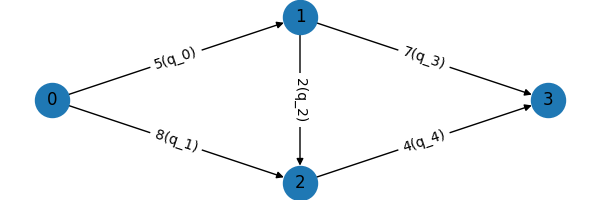
\includegraphics[scale=0.75]{primer_grafo/primer_grafo}
  \caption{Grafo del artículo original} \label{fig:primer_grafo/primer_grafo}
\end{figure}

\subsection{Resultados de Qiskit}
\label{sec:resultados-de-qiskit}
% TODOO: Hablar aquí sobre la diferencia entre los modificadores y la restricción extra
En las siguientes muestras se ha buscado replicar los resultados del artículo. Esto ha sido probado ya que, empleando los parámetros \(\beta = 0.28517317\) y \(\gamma = -5.05969577 \) dados como óptimos, se obtiene un gráfico muy similar al dado: \\

\begin{figure}[htbp]
  \centering
  \subfigure[Resultado del artículo]{
    \includegraphics[width=0.475\textwidth]{primer_grafo/sin_restriccion_extra/primer_paper_orig_resultado}
  }
  \subfigure[Resultado obtenido]{
    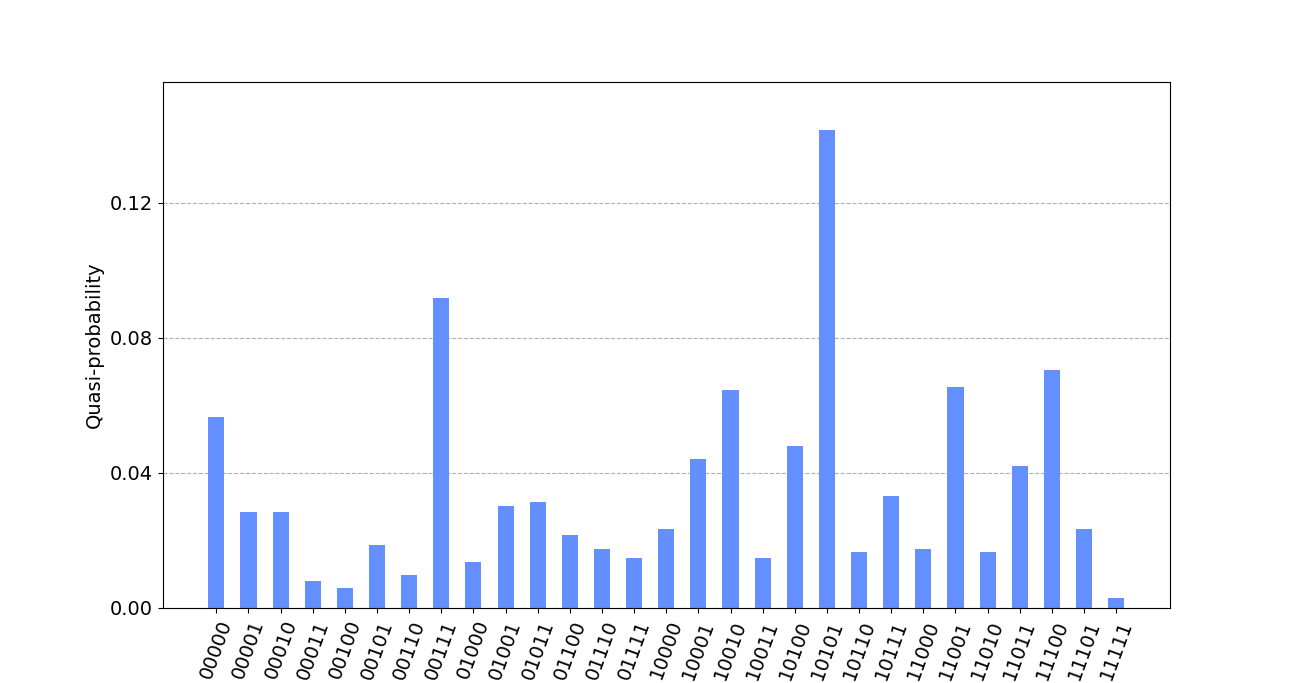
\includegraphics[width=0.475\textwidth]{primer_grafo/sin_restriccion_extra/primer_paper_aer_resultado}
  }
  \caption{} \label{fig:primer_grafo/sin_restriccion_extra/primer_paper_aer_resultado}
\end{figure}

De esta forma, se tiene que los resultados del artículo deberían ser equivalentes a los obtenidos en esta instancia del algoritmo.

\begin{table}[htbp]
  \centering
  \begin{tabular}{|c|r|r|}
    \hline
    \textbf{nº Capas} & \textbf{Estadística máxima (\%)} & \textbf{Estadística global (\%)} \\ \hline
    p = 1 & 91.3\% & 39.34\% \\ \hline
    p = 2 & 64.6\% & 24.16\% \\ \hline
    p = 3 & 63.4\% & 18.82\% \\ \hline
  \end{tabular}
  \caption{Resultados de la ejecución de la versión de QAOA del artículo}
  \label{tab:primer_paper_aer_estadisticas}
\end{table}

El primer resultado notable en la tabla \ref{tab:primer_paper_aer_estadisticas} es un empeoramiento de los resultados a medida que se aumenta el número de capas, lo cual es contrario a lo esperado teóricamente. \\
% TODOOOOO: Esto tiene que estar mal, lo muestro de todas formas? (el hecho de que al aumentar p empeore el algoritmo)
Además, la gran diferencia entre los resultados dados por la estadística máxima y la estadística global denotan una gran cantidad de ruido al ejecutar el algoritmo, lo cual se corrobora viendo los resultados de ejecuciones concretas, como los dados en la figura \ref{fig:primer_grafo/sin_restriccion_extra/primer_paper_aer_resultado}. \\

El resultado de la función gamma es el siguiente:
\begin{figure}[htbp]
  \centering
  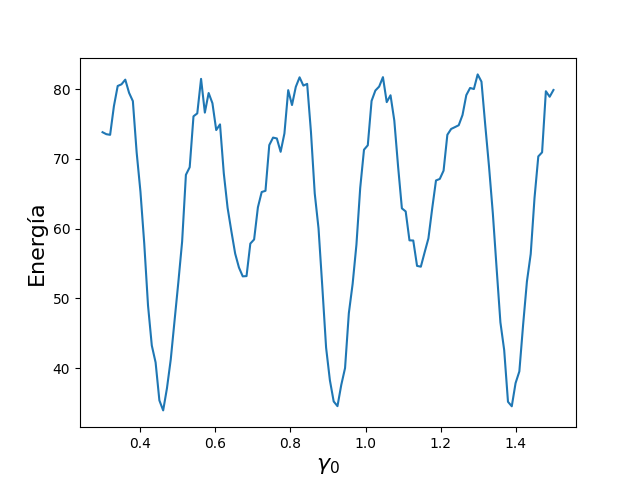
\includegraphics[scale=0.5]{primer_grafo/sin_restriccion_extra/primer_paper_p_27_gamma_fun}
  \caption{Función gamma. Caso del artículo}
  \label{fig:primer_grafo/sin_restriccion_extra/primer_paper_p_27_gamma_fun}
\end{figure}

Se puede ver que existen un gran número de mínimos locales, lo cual dificulta la tarea del optimizador clásico. Esto se corrobora ya que, al inicializar los parámetros como \(\beta = 1.0 \ \gamma = 0.5\), para \(p = 1\) se obtiene el camino óptimo el 100\% de las ejecuciones. \\
% TODO: Comparar esta función gamma con la que aparece en MAX-CUT, esto estará en el anexo
Este proceso de inicializar los parámetros con valores concretos no sería una solución válida, ya que se trata de una metodología no automática en la que, para ejecutar correctamente el algoritmo, se necesitaría conocer antes su propio resultado. Además la ejecución correcta sucede para \(p = 1\), pero al igual que el caso por defecto (\(\beta = 1.0 \ \gamma = 1.0\)), no escala correctamente al aumentar el número de capas.


\subsection{Resultados de D-Wave}
\label{sec:resultados-de-qiskit}
Con respecto a los resultados de aplicar Quantum Annealing utilizando los sistemas de D-Wave se ha obtenido el resultado de la tabla \ref{tab:primer_paper_dwave_estadisticas}

\begin{table}[htbp]
  \centering
  \begin{tabular}{|c|r|r|}
    \hline
    \textbf{Camino} & \textbf{Energía} & \textbf{Número de ocurrencias} \\ \hline
    10101 (\textbf{Óptimo}) & 11 & 348 \\ \hline
    01001 & 12 & 373 \\ \hline
    10010 & 12 & 294 \\ \hline
    00000 & 54 &   4 \\ \hline
    00001 & 58 &   1 \\ \hline
    10000 & 59 &   1 \\ \hline
    00101 & 60 &   1 \\ \hline
    10100 & 61 &   1 \\ \hline
    01010 & 69 &   1 \\ \hline
  \end{tabular}
  \caption{Resultados de la ejecución del grafo del artículo en D-Wave}
  \label{tab:primer_paper_dwave_estadisticas}
\end{table}

La energía se refiere al coste de dicho camino de acuerdo con la función de coste utilizada. Se puede ver cómo, aunque se encuentre el camino óptimo un menor número de veces que en QAOA, existe una mayor coherencia en los resultados. Esto es así porque los caminos con mayores ocurrencias son los que tienen menor energía, mientras en las ejecuciones de Qiskit se pueden ver ejemplos, como es el camino 00111 en la figura \ref{fig:primer_grafo/sin_restriccion_extra/primer_paper_aer_resultado} con un gran número de ocurrencias pero también una energía elevada.
\footnote{En la ejecución de Qiskit, la energía del camino ``00111'' es 150. Esto se debe a que se rompen varias restricciones presentes en la función de coste. Este valor puede variar dependiendo del multiplicador de Lagrange empleado
  % TODO: Citar multiplicador de lagrange del anexo
  y las restricciones utilizadas.}

\end{document}
%%% Local Variables:
%%% mode: latex
%%% TeX-master: t
%%% End:
